\documentclass[10pt,twocolumn]{article}

\usepackage[margin=1.9cm,columnsep=0.7cm]{geometry}
\usepackage[utf8]{inputenc}
\usepackage[T1]{fontenc}
\usepackage{times}
\usepackage{graphicx}
\usepackage{booktabs}
\usepackage{caption}
\usepackage{float}
\usepackage{xcolor}
\usepackage{hyperref}
\hypersetup{colorlinks=true, linkcolor=blue!50!black, urlcolor=blue!50!black, citecolor=blue!50!black}
\usepackage{titlesec}
\usepackage{abstract}
\usepackage{enumitem}
\setlist{noitemsep}

\titleformat{\section}{\normalfont\large\bfseries}{\thesection}{0.6em}{}
\titleformat{\subsection}{\normalfont\bfseries}{\thesubsection}{0.6em}{}
\titlespacing{\section}{0pt}{10pt}{4pt}
\titlespacing{\subsection}{0pt}{8pt}{3pt}

\renewcommand{\abstractnamefont}{\normalfont\bfseries}
\renewcommand{\abstracttextfont}{\normalfont\itshape}
\renewcommand{\abstractname}{Resumo}

\title{\vspace{-1.2em}\textbf{Observatório do Mercado de Trabalho em Ciência de Dados no Brasil:\\
Coleta Multi-Fonte, Unificação de Dados e Análise Salarial}}

\author{
Richard Elias Soares Viana\\
\small Observatório de Empregos --- Extensão IMPA-Tech\\
\small \texttt{erichardsv1234@gmail.com}
}
\date{Julho de 2026}

\begin{document}
\twocolumn[
  \begin{@twocolumnfalse}
    \maketitle
    \begin{abstract}
    \noindent
    Este relatório descreve a arquitetura de coleta, unificação e limpeza de dados do
    \emph{Job Data Observatory}, um sistema de código aberto que consolida vagas e
    referências salariais de Ciência de Dados no Brasil a partir de cinco fontes
    heterogêneas (LinkedIn, Glassdoor, Catho, portais Gupy e uma base curada
    manualmente), e apresenta a análise mais recente do mercado gerada a partir dessa
    base unificada. Descrevemos a metodologia de normalização de esquema, a
    classificação de cargo/senioridade por vocabulário de expressões regulares
    compartilhado entre fontes, e um conjunto de correções de qualidade de dados
    identificadas durante a auditoria do pipeline (falsos positivos de regex,
    colunas de origem corrompidas e valores salariais implausíveis). A base
    unificada resultante contém 5.252 registros, com cobertura de salário de 97,5\%
    (ante 3,2\% antes da integração das fontes adicionais). Os resultados mostram uma
    progressão salarial de quase 10$\times$ entre estágio e posições de staff, uma
    concentração de vagas em São Paulo, e um prêmio salarial de 58\% para vagas
    remotas frente a presenciais. Discutimos as limitações da amostra, em particular
    o viés de composição entre vagas individuais e referências agregadas de
    salário.

    \medskip\noindent
    \textbf{Palavras-chave:} mercado de trabalho, ciência de dados, engenharia de
    dados, unificação de dados, análise salarial, Brasil.
    \end{abstract}
    \vspace{1em}
  \end{@twocolumnfalse}
]

\section{Introdução}

O mercado brasileiro de Ciência de Dados carece de fontes de dados públicas,
atualizadas e consolidadas sobre remuneração, distribuição geográfica e
modalidade de trabalho. Portais de emprego e de referência salarial (LinkedIn,
Glassdoor, Catho, plataformas baseadas em Gupy) publicam informações parciais,
em formatos distintos e sem interoperabilidade entre si. O \emph{Job Data
Observatory} foi criado como projeto de extensão do IMPA-Tech para preencher
essa lacuna: um sistema que coleta dados de múltiplas fontes, os normaliza para
um esquema unificado, e os disponibiliza por meio de um painel interativo e um
mecanismo de busca semântica.

Este relatório tem dois objetivos. Primeiro, documentar a metodologia de coleta
e unificação de dados, incluindo um conjunto de correções de qualidade
aplicadas durante uma auditoria completa do pipeline --- a maioria das fontes
manualmente coletadas (\texttt{data\_preprocess/}) estava, até esta revisão,
coletada mas nunca efetivamente incorporada à base final. Segundo, apresentar
a análise mais atual do mercado, obtida a partir da base unificada resultante.

\section{Metodologia}

\subsection{Fontes de Dados}

A base unificada combina cinco fontes independentes, cada uma processada por um
carregador dedicado que mapeia seus campos originais para um esquema comum de
16 colunas (\texttt{company}, \texttt{role}, \texttt{seniority}, \texttt{region},
\texttt{work\_model}, \texttt{contract\_type}, \texttt{salary}, entre outras). A
Tabela~\ref{tab:sources} resume a composição da base.

\begin{table}[H]
\centering
\small
\caption{Composição da base unificada por fonte.}
\label{tab:sources}
\begin{tabular}{@{}lrl@{}}
\toprule
\textbf{Fonte} & \textbf{Registros} & \textbf{Natureza} \\
\midrule
Glassdoor & 4.698 & Referência salarial agregada \\
Salário Transparente & 497 & Vaga individual \\
Portais Gupy & 41 & Vaga individual \\
Catho & 16 & Vaga individual \\
\midrule
\textbf{Total} & \textbf{5.252} & --- \\
\bottomrule
\end{tabular}
\end{table}

O LinkedIn (\texttt{job\_scrapper/}) é uma sexta fonte planejada, coletada via
Selenium; como exige uma sessão autenticada e está sujeita aos termos de uso da
plataforma, o pipeline de unificação foi projetado para funcionar
\emph{sem} essa fonte --- caso o arquivo de coleta não exista, o carregador
correspondente é ignorado com um aviso, em vez de interromper todo o processo.

Note-se que 89,4\% dos registros vêm do Glassdoor, que reporta \emph{benchmarks}
de salário por combinação empresa/cargo, não vagas abertas no momento da
coleta. Essas linhas são mantidas 1:1 (não expandidas pelo número de relatos
salariais subjacente) para evitar distorção nas estatísticas de contagem de
vagas, mas isso implica que a base mistura duas naturezas de registro distintas
--- ponto retomado na Seção~\ref{sec:limitacoes}.

\subsection{Pipeline de Unificação}

O módulo \texttt{data\_treatment/merge\_data\_sources.py} orquestra a
unificação em três etapas: (i) carregamento e normalização por fonte; (ii)
classificação de \texttt{role} e \texttt{seniority} por vocabulário de
expressões regulares compartilhado (\texttt{ROLE\_REGEX}, \texttt{SENIORITY\_REGEX})
entre todas as fontes, garantindo que a mesma vaga produza o mesmo rótulo
independentemente de sua origem; e (iii) binarização da coluna
\texttt{benefits} em colunas booleanas (\texttt{benefit\_<nome>}) para consumo
direto pelo painel.

Antes desta revisão, apenas a fonte \emph{Salário Transparente} normalizava
\texttt{role} pelo vocabulário compartilhado; as demais gravavam o cargo bruto
em português, fragmentando os gráficos por cargo em dezenas de rótulos
equivalentes (p.ex. ``Analista de Dados Sênior'' e ``Data Analyst'' como
categorias distintas). A normalização foi estendida a todas as fontes.

\subsection{Auditoria e Correções de Qualidade}

A integração das fontes adicionais expôs três problemas de qualidade,
corrigidos nesta revisão:

\begin{enumerate}
\item \textbf{Falso positivo geográfico.} O padrão de regex para o estado do
  Pará (\texttt{par[áa]|pa}) também casa com a preposição portuguesa ``para'',
  produzindo detecções incorretas de estado ao ser aplicado sobre texto livre
  (descrições de vaga). A extração de região foi restrita a campos
  estruturados de localização.
\item \textbf{Coluna de origem corrompida.} A coluna \texttt{empresa} do
  Catho continha texto de interface (``compartilhar'', ``Idioma:'') em vez do
  nome da empresa, artefato do seletor CSS usado na coleta manual; a coluna é
  descartada nesta fonte em vez de propagar dados incorretos.
\item \textbf{Valores salariais implausíveis.} Um pequeno subconjunto de
  registros do Glassdoor (82 de 4.698) reportava salário médio mensal acima de
  R\$~100.000 --- provavelmente remuneração anual rotulada como mensal na
  fonte original. Esses valores são tratados como ausentes em vez de
  distorcer as distribuições salariais.
\end{enumerate}

\subsection{Vetorização Semântica}

Para a busca semântica (\texttt{/api/search}), cada registro é convertido em
uma representação textual combinando cargo, senioridade, região, modalidade,
tecnologias, benefícios e uma versão truncada da descrição, codificada pelo
modelo multilíngue \texttt{paraphrase-multilingual-mpnet-base-v2}
(\emph{sentence-transformers}) em vetores de 768 dimensões. Consultas do
usuário são codificadas no mesmo espaço e ranqueadas por similaridade de
cosseno contra a matriz de embeddings.

\section{Resultados}

\subsection{Cobertura de Dados}

A integração das fontes adicionais elevou a cobertura de salário de 3,2\%
(497 de 15.436 registros, estado anterior da base) para 97,5\%
(5.123 de 5.252). Localização e modalidade de trabalho, por virem
majoritariamente de fontes manuais, têm cobertura bem menor: 9,9\% e 10,3\%,
respectivamente. A base cobre 2.483 empresas distintas.

\subsection{Salário por Senioridade}

A Tabela~\ref{tab:seniority} e a Figura~\ref{fig:salario} mostram a progressão
salarial por nível. A diferença entre estágio (R\$~2.813) e posições de staff
(R\$~27.941) é de quase 10$\times$. O salto mais expressivo em termos
proporcionais ocorre entre júnior e sênior (2,45$\times$).

\begin{table}[H]
\centering
\small
\caption{Salário base por nível de senioridade.}
\label{tab:seniority}
\begin{tabular}{@{}lrrr@{}}
\toprule
\textbf{Nível} & \textbf{n} & \textbf{Média (R\$)} & \textbf{Mediana (R\$)} \\
\midrule
Estágio              & 76  & 2.813  & 2.000 \\
Júnior                & 865 & 5.646  & 5.000 \\
Pleno                 & 670 & 8.695  & 8.000 \\
Sênior                & 875 & 13.805 & 13.000 \\
Líder/Coordenador     & 54  & 19.163 & 18.000 \\
Gerente               & 68  & 23.800 & 21.500 \\
Staff                 & 17  & 27.941 & 23.000 \\
\midrule
Não informado         & 2.493 & 9.072 & 7.000 \\
\bottomrule
\end{tabular}
\end{table}

\begin{figure}[H]
\centering
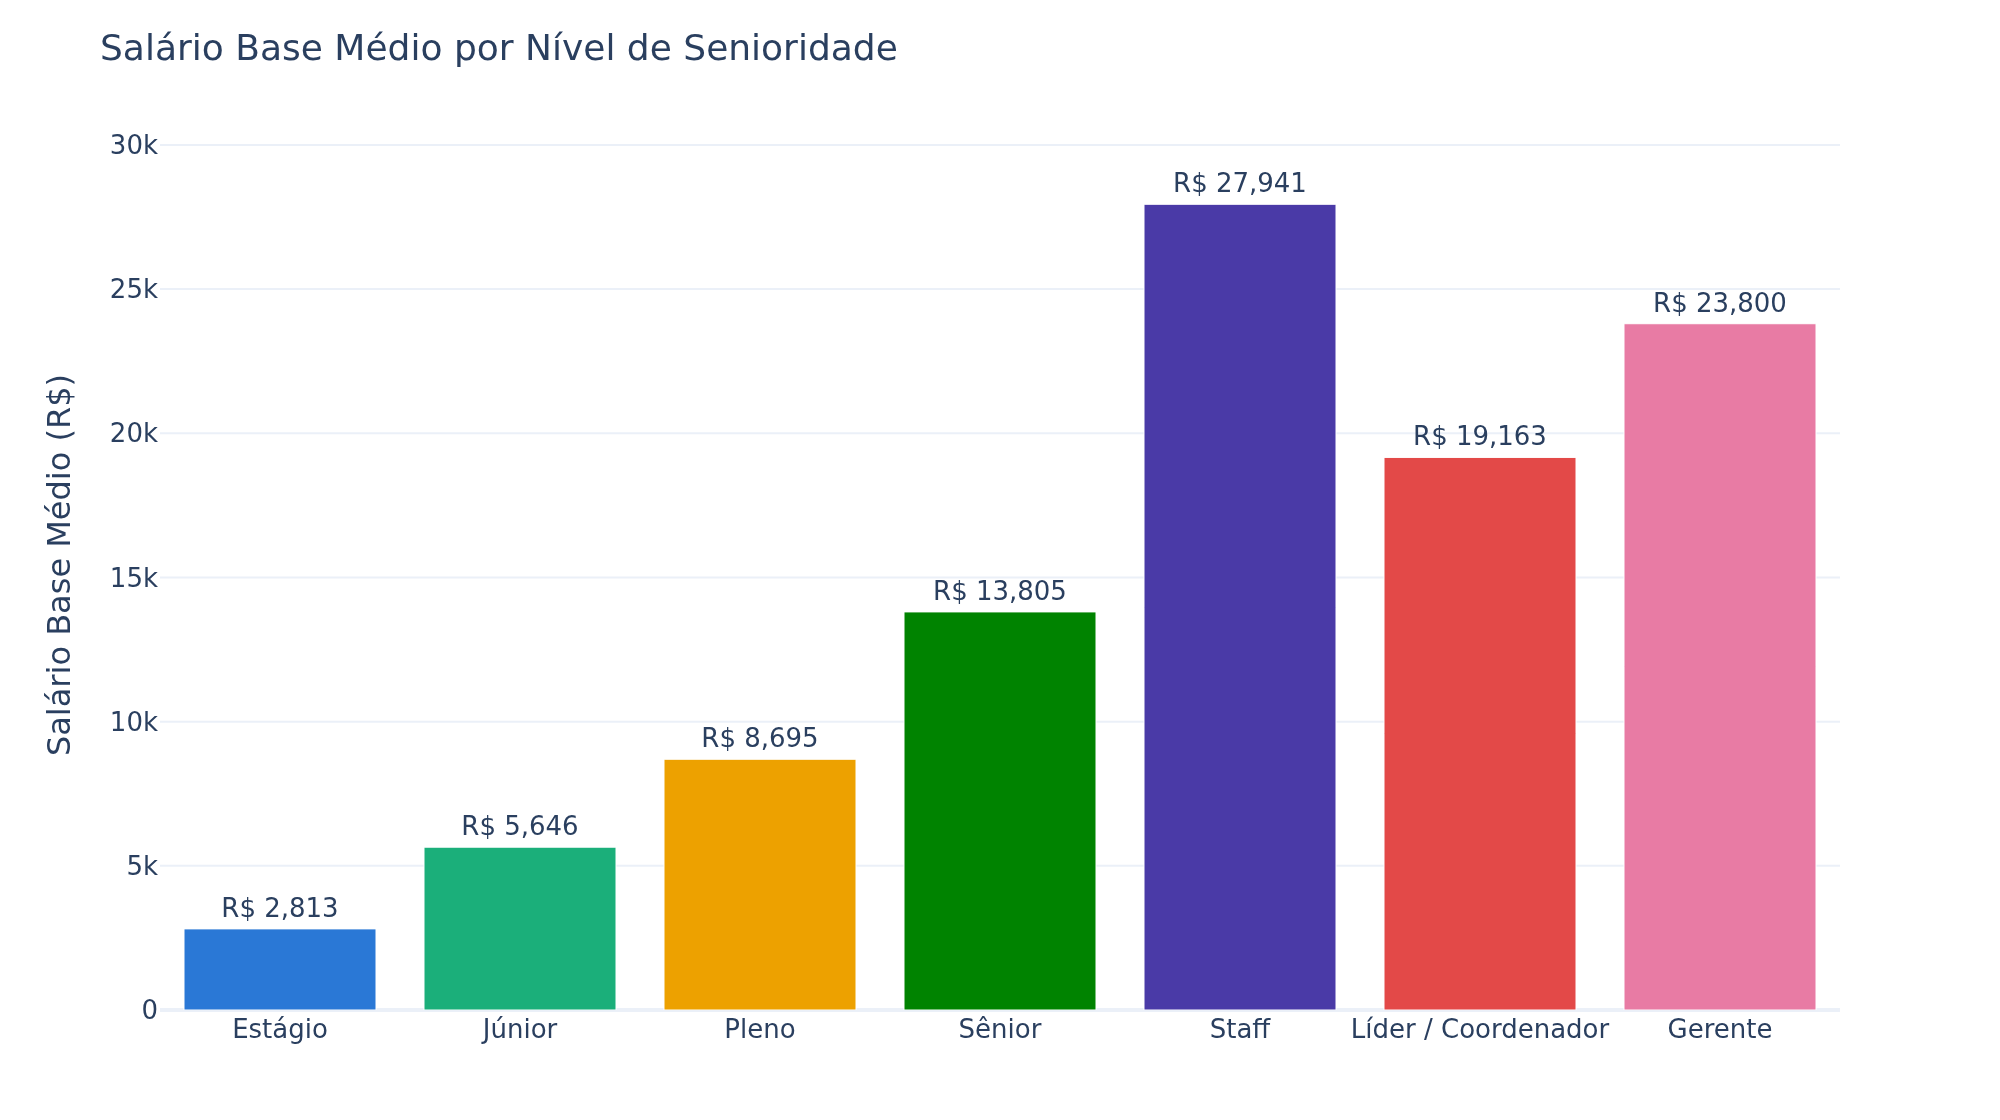
\includegraphics[width=\linewidth]{figures/salario_por_nivel.png}
\caption{Salário base médio por nível de senioridade.}
\label{fig:salario}
\end{figure}

\subsection{Distribuição Geográfica}

Entre os 520 registros que informam localização (Tabela~\ref{tab:estados}), São
Paulo concentra 57\% das vagas geolocalizadas. Santa Catarina apresenta o
maior salário médio entre os estados com amostra relevante, embora com apenas
17 registros.

\begin{table}[H]
\centering
\small
\caption{Top 8 estados por número de registros.}
\label{tab:estados}
\begin{tabular}{@{}lrrr@{}}
\toprule
\textbf{Estado} & \textbf{n} & \textbf{Média (R\$)} & \textbf{Mediana (R\$)} \\
\midrule
São Paulo        & 280 & 9.799  & 9.000 \\
Rio de Janeiro    & 64  & 9.224  & 9.025 \\
Minas Gerais      & 47  & 8.672  & 7.500 \\
Paraná            & 38  & 7.079  & 6.500 \\
Santa Catarina    & 17  & 11.834 & 8.000 \\
Pernambuco        & 10  & 6.668  & 5.650 \\
Ceará             & 9   & 6.770  & 5.796 \\
Distrito Federal  & 9   & 8.193  & 8.000 \\
\bottomrule
\end{tabular}
\end{table}

\subsection{Modalidade de Trabalho}

Entre os 541 registros que informam modalidade (Tabela~\ref{tab:modalidade},
Figura~\ref{fig:modalidade}), vagas remotas pagam, em média, 58\% a mais que
vagas presenciais (R\$~10.081 vs.\ R\$~6.372).

\begin{table}[H]
\centering
\small
\caption{Salário base por modalidade de trabalho.}
\label{tab:modalidade}
\begin{tabular}{@{}lrrr@{}}
\toprule
\textbf{Modalidade} & \textbf{n} & \textbf{Média (R\$)} & \textbf{Mediana (R\$)} \\
\midrule
Remoto      & 270 & 10.081 & 9.000 \\
Híbrido      & 191 & 9.060  & 8.270 \\
Presencial  & 75  & 6.372  & 5.276 \\
\bottomrule
\end{tabular}
\end{table}

\begin{figure}[H]
\centering
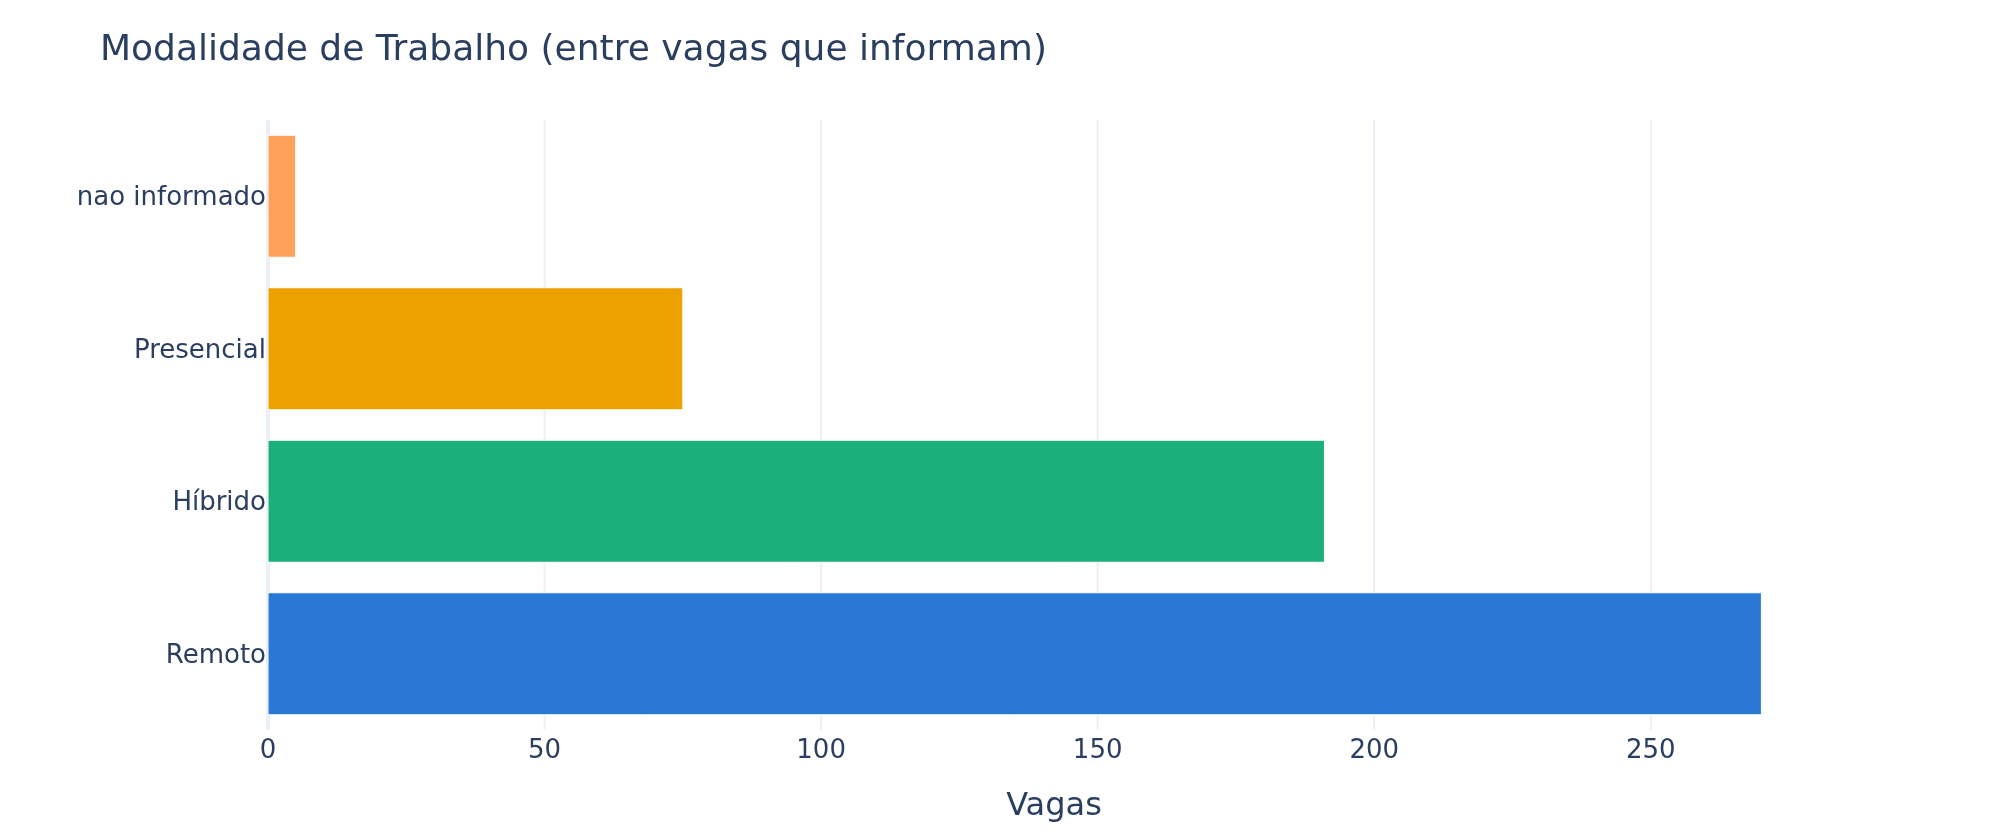
\includegraphics[width=\linewidth]{figures/modalidade.png}
\caption{Distribuição de vagas por modalidade de trabalho.}
\label{fig:modalidade}
\end{figure}

\subsection{Empresas e Benefícios}

Bancos de grande porte (Bradesco, Itaú), varejo digital (iFood, Mercado Livre)
e consultorias (Accenture, IBM) lideram em número de registros
(Figura~\ref{fig:empresas}), refletindo tanto o tamanho dessas operações
quanto sua presença consolidada em bases de referência salarial.

\begin{figure}[H]
\centering
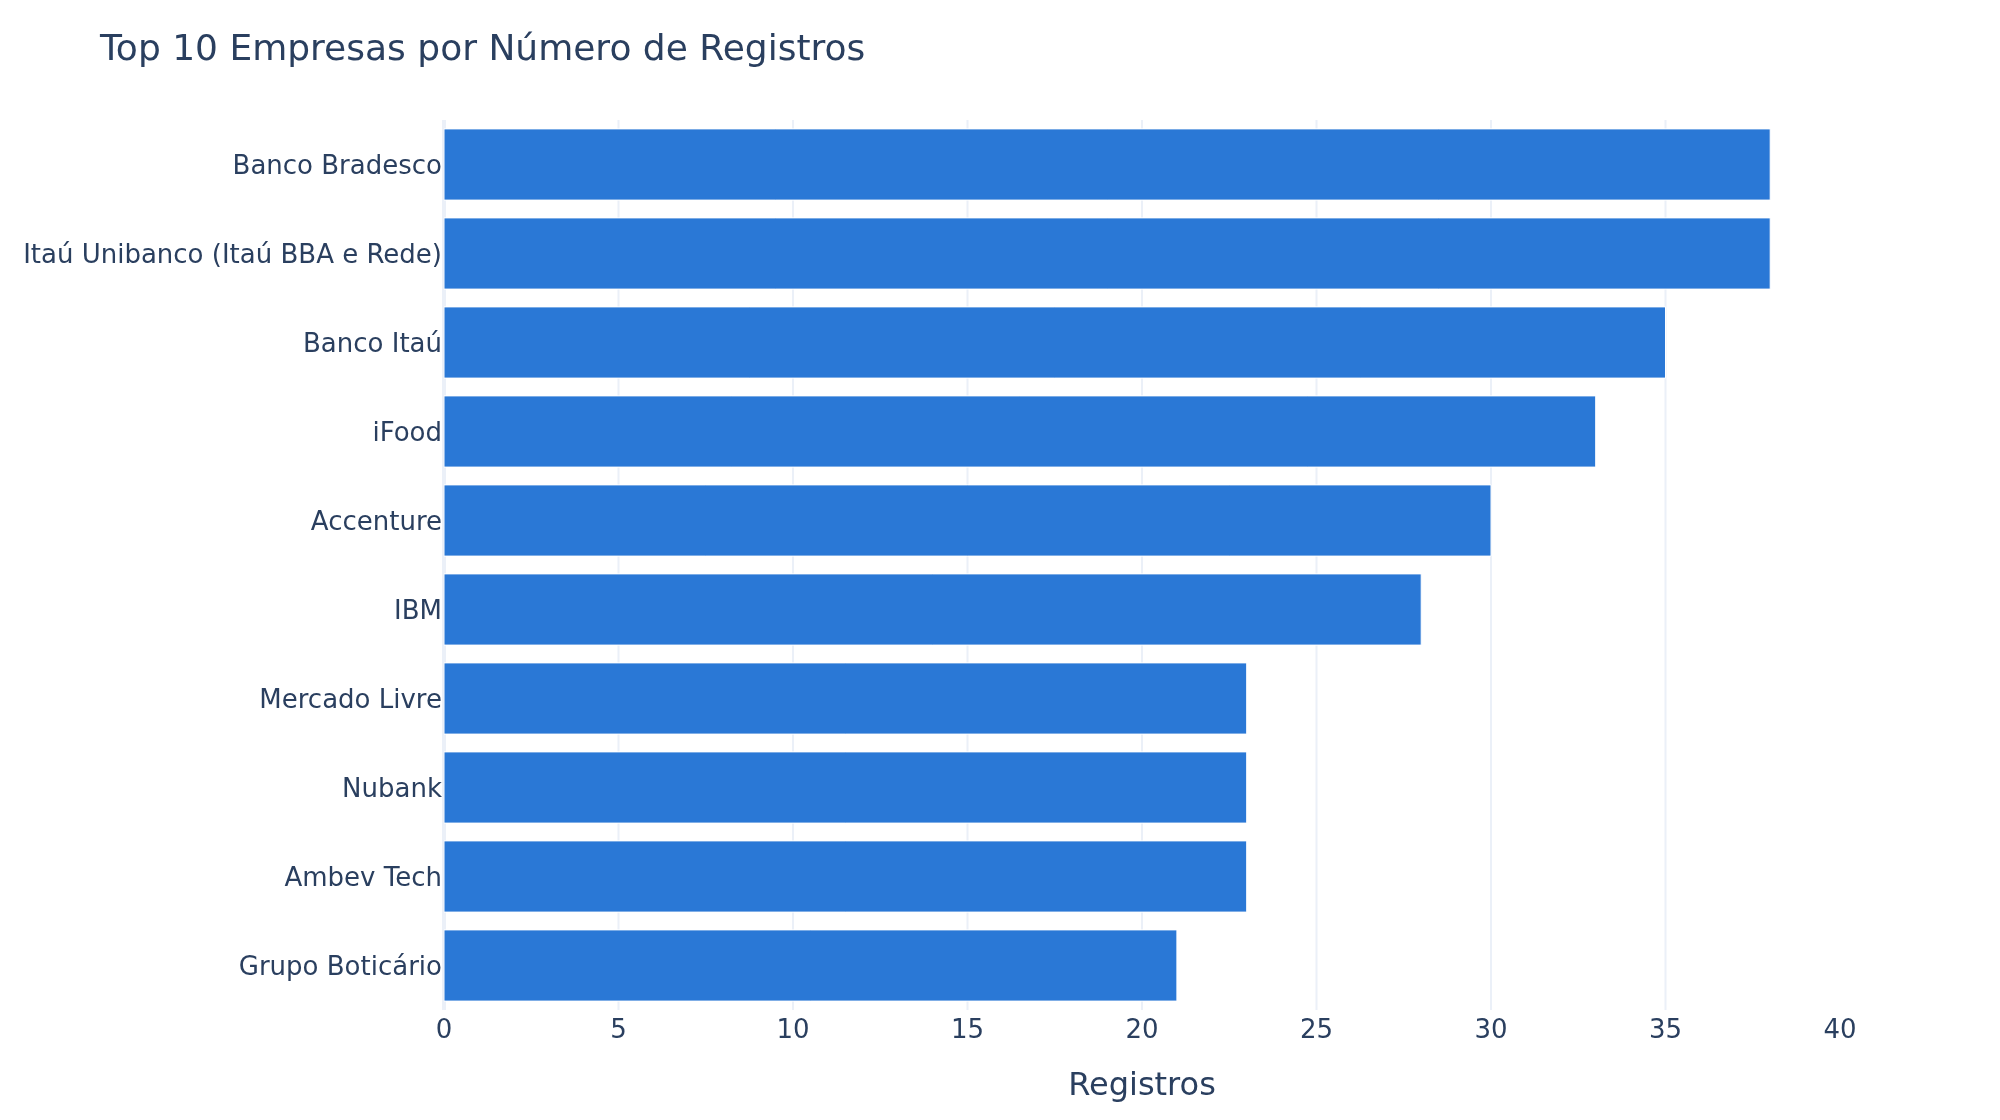
\includegraphics[width=\linewidth]{figures/top_empresas.png}
\caption{Top 10 empresas por número de registros.}
\label{fig:empresas}
\end{figure}

Entre as 542 vagas que detalham benefícios, plano de saúde (79,0\%), Gympass
(72,3\%) e vale-refeição (71,6\%) são os mais recorrentes
(Figura~\ref{fig:beneficios}).

\begin{figure}[H]
\centering
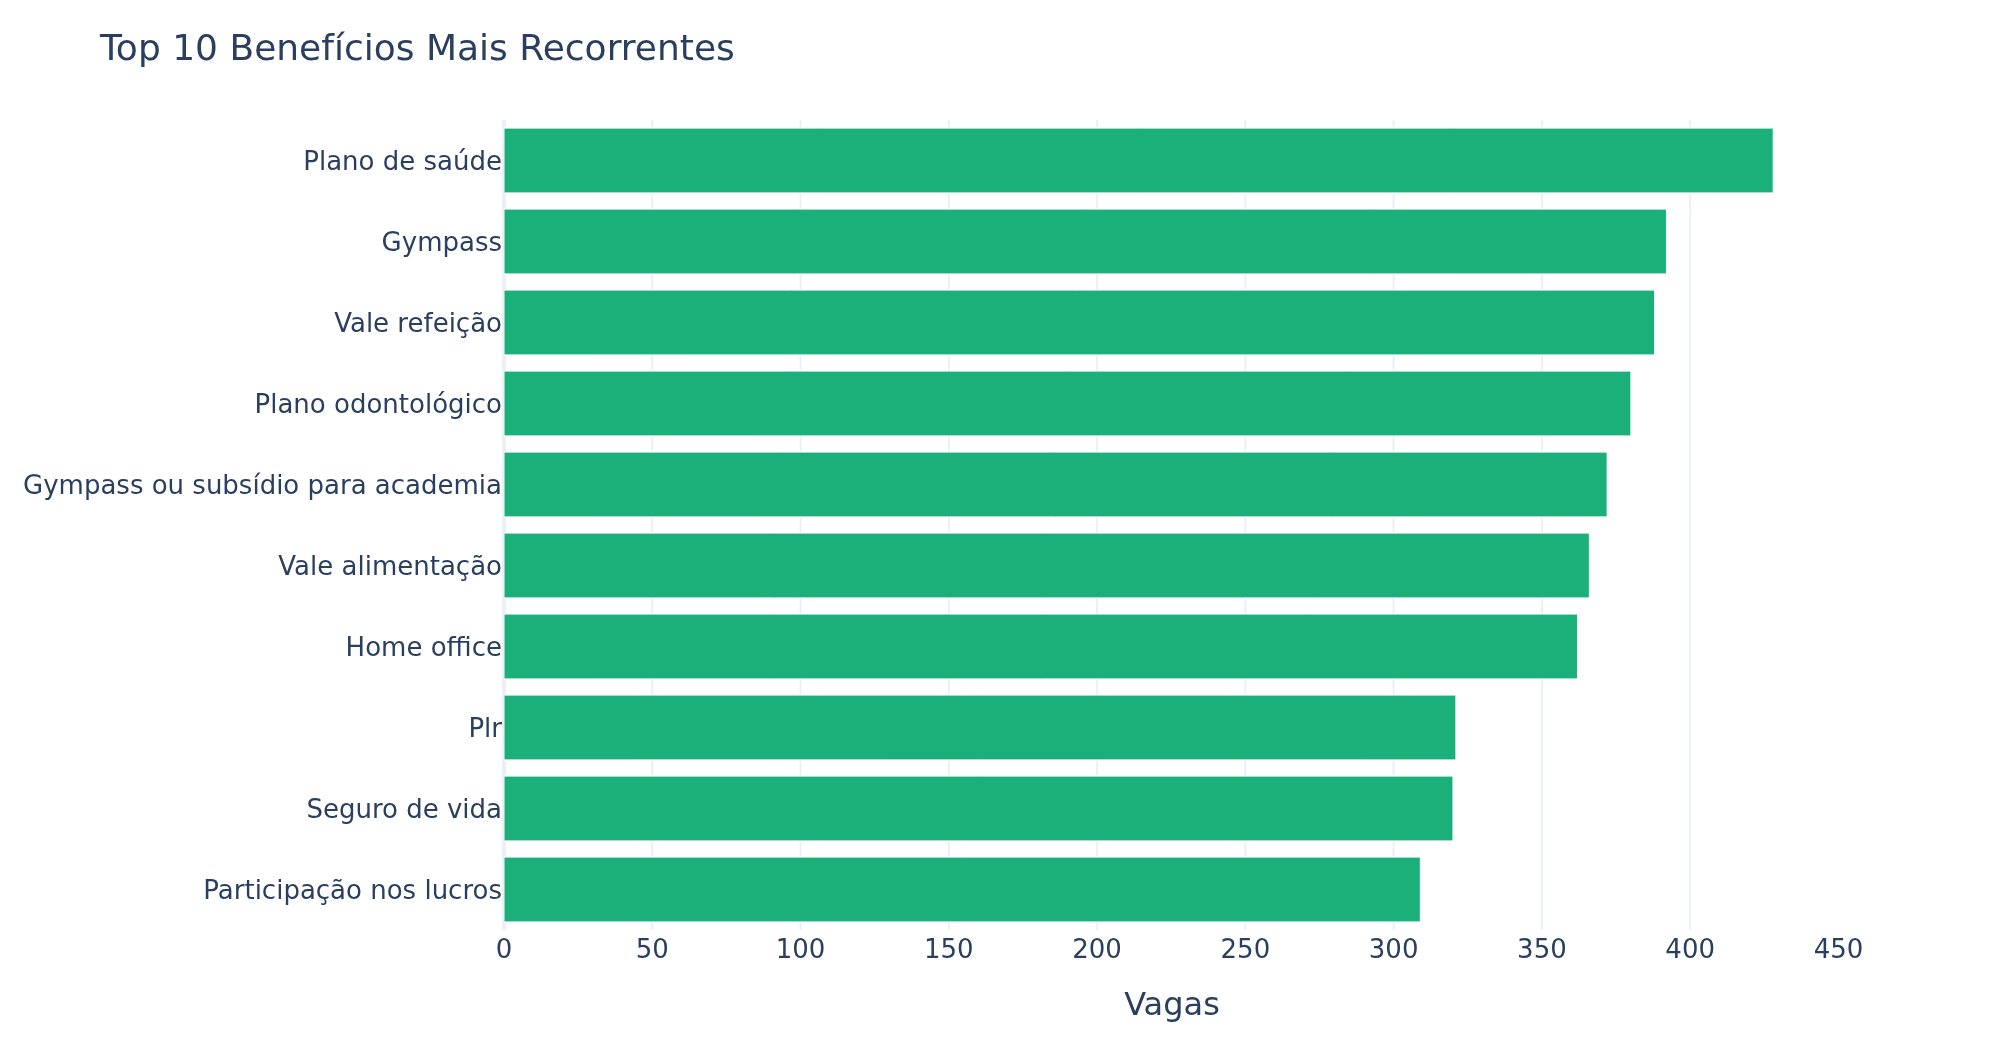
\includegraphics[width=\linewidth]{figures/top_beneficios.png}
\caption{Top 10 benefícios mais recorrentes.}
\label{fig:beneficios}
\end{figure}

\section{Discussão e Limitações}
\label{sec:limitacoes}

Três limitações merecem destaque para uma leitura criteriosa dos resultados.
Primeiro, a base mistura vagas individuais com \emph{benchmarks} agregados do
Glassdoor (89,4\% dos registros); estes últimos refletem estimativas de
remuneração por empresa/cargo, não necessariamente posições abertas no momento
da coleta. Segundo, a cobertura de campos é desigual: enquanto salário está
presente em 97,5\% dos registros, localização, modalidade e benefícios cobrem
apenas ${\sim}10\%$, concentrados nas fontes manuais. Terceiro, a amostra é
fortemente enviesada para o cargo de Cientista de Dados (92,9\% dos registros),
refletindo o escopo de coleta do observatório e da consulta usada no
Glassdoor, não a proporção real desses cargos no mercado de tecnologia como um
todo. Grupos com poucas observações (Staff, $n=17$; Líder/Coordenador,
$n=54$) devem ser interpretados como direcionais.

\section{Conclusão}

A auditoria e extensão do pipeline de unificação elevaram a cobertura de
salário da base de 3,2\% para 97,5\%, ao integrar três fontes manualmente
coletadas que não estavam sendo aproveitadas, e corrigiram três problemas
concretos de qualidade de dados (falso positivo geográfico, coluna de origem
corrompida, outliers salariais implausíveis). A análise resultante confirma
padrões esperados do mercado brasileiro de dados --- progressão salarial
acentuada por senioridade, concentração em São Paulo, prêmio para trabalho
remoto --- com transparência explícita sobre o tamanho de amostra por
indicador. Trabalhos futuros devem priorizar a retomada da coleta via
LinkedIn e a incorporação das submissões manuais (\texttt{/vaga/nova}) ao
pipeline de unificação, hoje armazenadas separadamente.

\vspace{0.5em}
\noindent\textit{Código-fonte, dados e o painel interativo completo estão
disponíveis no repositório do projeto.}

\end{document}
